% Chapter 3

\chapter{前端设计与实现}

\section{概述}

网站主要采用W3 CSS样式进行修饰,主要使用灰白黑三种颜色,风格较为简约、清爽。整个网站系统包含欢迎界面、主界面、登录界面、注册界面、文件详情页面等共计12个子页面。

图\ref{fig:link}展示了12个子页面之间的链接跳转关系。页面之间的跳转关系有简单的直接跳转,也有经过服务器校验后返回的重定向跳转。而对于有些需要校验用户输入正确性的页面,如果服务器端校验失败,一般会重定向回原页面,并附带上相应的错误提示信息。图中以蓝色虚线作为分隔标志,访问蓝色虚线左侧的页面无需用户处于登录状态,而访问蓝色虚线右侧的页面则要求用户必须处于登录状态,否则服务器将自动把用户重定向到登录界面。

\begin{figure}[!htb]
	\centering
	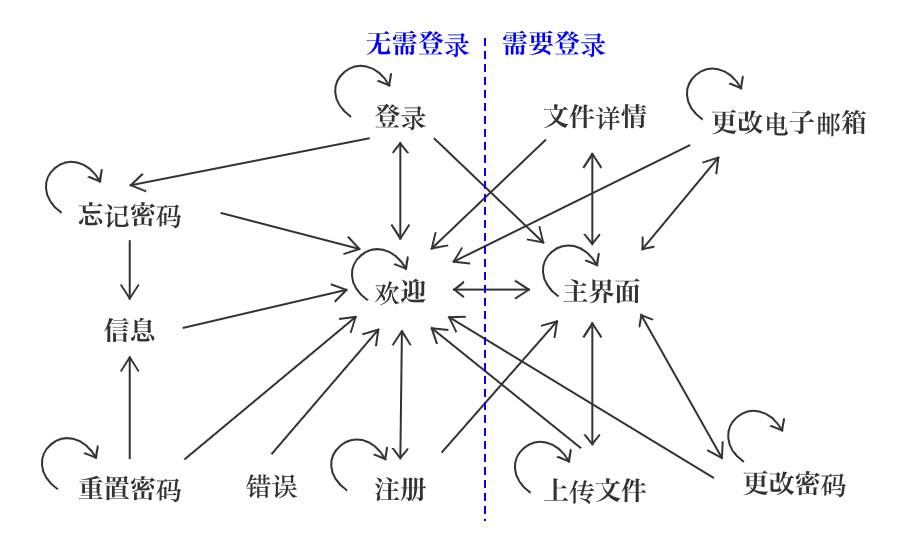
\includegraphics[width=0.8\textwidth]
	{figures/link-cn.png}\\
	\caption{子页面间的链接跳转关系}
	\label{fig:link}
\end{figure}

\section{欢迎界面}

欢迎界面是用户打开本系统所看到的第一个页面,即本系统的门户,如图\ref{fig:index}所示。

欢迎界面的上方是本系统的名称——SigDict。同时这部分也是本系统公用的,这部分将重复出现于后续的所有界面中。同时,通过点击这部分界面的“SigDict”链接,可以跳转到欢迎界面中。因此本项目中所有的子页面都可以直接跳转到欢迎界面。

欢迎界面的左侧是一片小短文,其中简要解释了本项目的起源、特性以及简要用途。

欢迎界面的右侧有引导用户登录和注册的按钮,用户点击后会分别打开两个新的页面,完成登录或者注册的操作。

\begin{figure}[!htb]
	\centering
	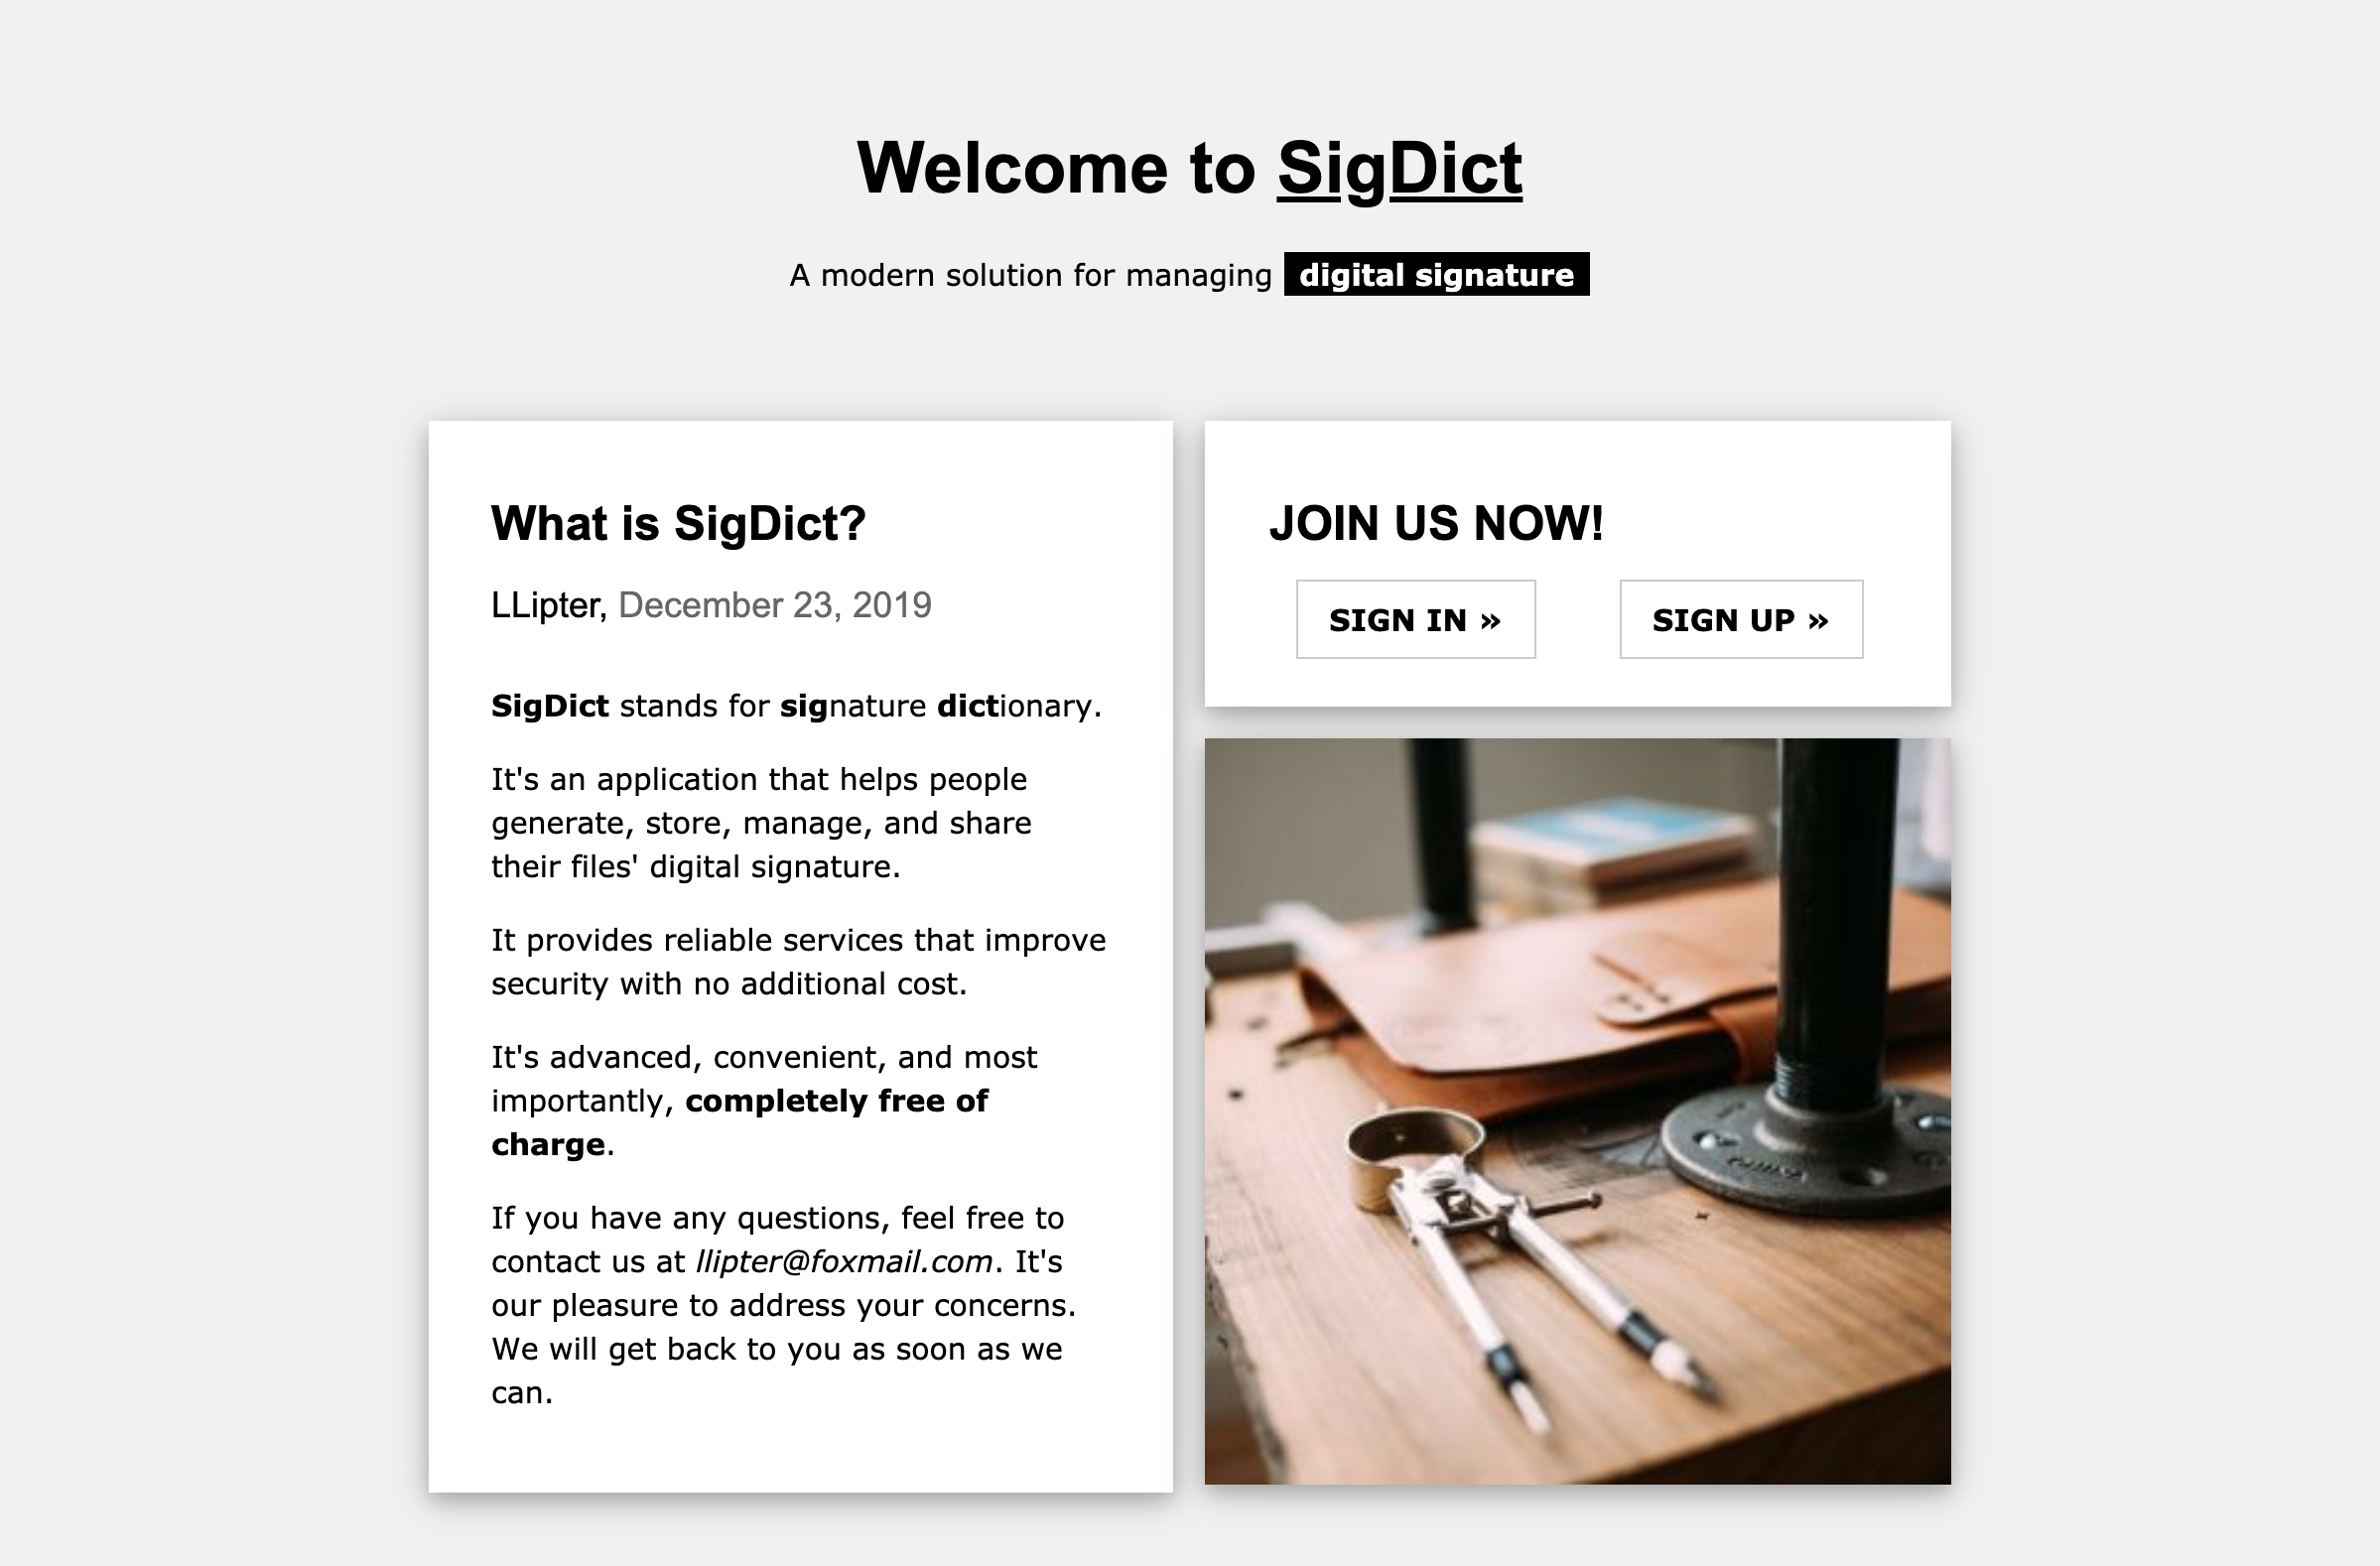
\includegraphics[width=0.8\textwidth]
	{figures/index.png}\\
	\caption{欢迎界面}
	\label{fig:index}
\end{figure}

\section{登录和注册界面}

在登录界面(图\ref{fig:login})中,用户需要输入用户名和密码,在校验正确后即可成功登录。而如果用户忘记密码可以点击“FORGET PASSWORD”,通过验证过的邮箱重置密码。

在注册界面(图\ref{fig:register})中,用户需要输入用户名、电子邮箱地址、密码、第二次密码确认这四项信息。在上述四项信息全部校验正确后注册成功,并跳转到主界面。校验规则将在小节\ref{sec:registerV}中具体介绍。

\begin{figure}[!htb]
	\begin{minipage}[t]{0.5\textwidth}
		\centering
		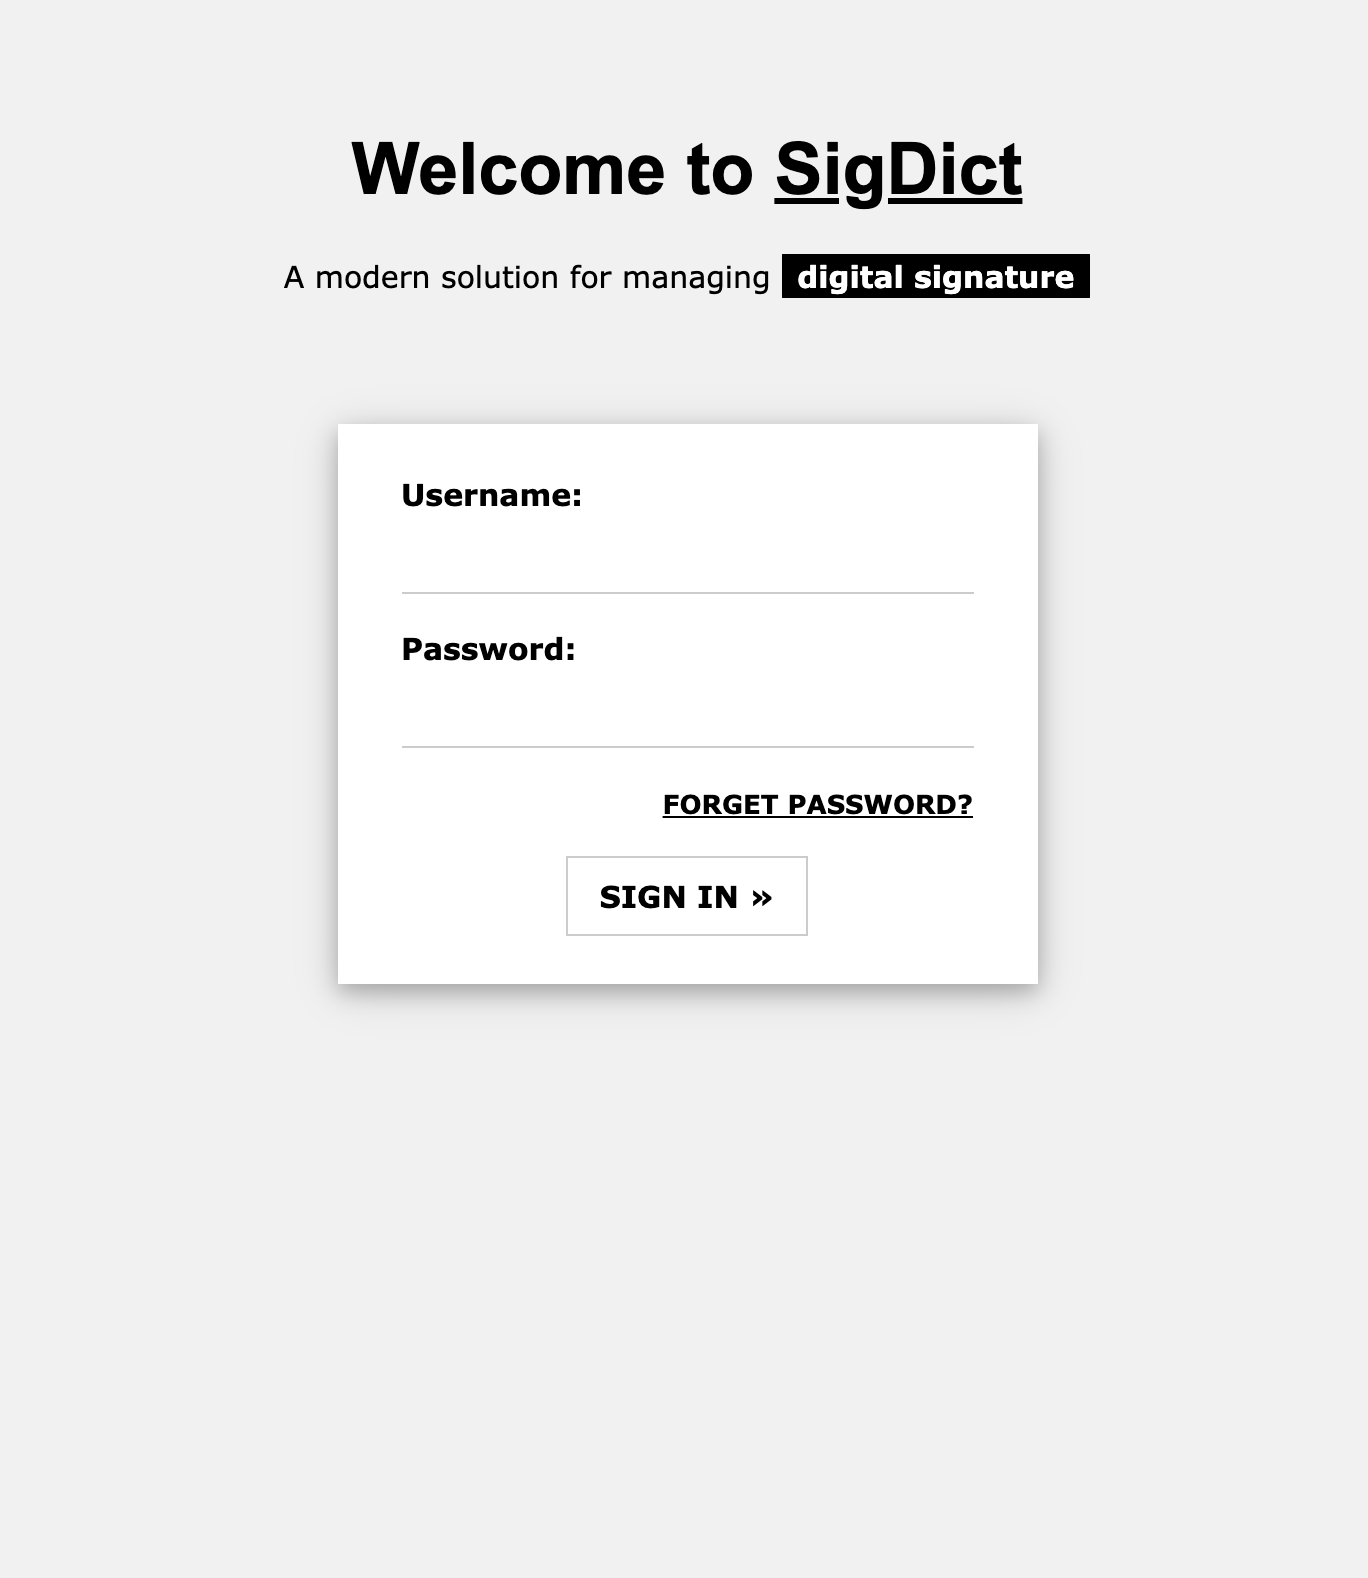
\includegraphics[width=1\textwidth]
		{figures/login.png}\\
		\caption{登录界面}
		\label{fig:login}
	\end{minipage}
	\qquad
	\begin{minipage}[t]{0.5\textwidth}
		\centering
		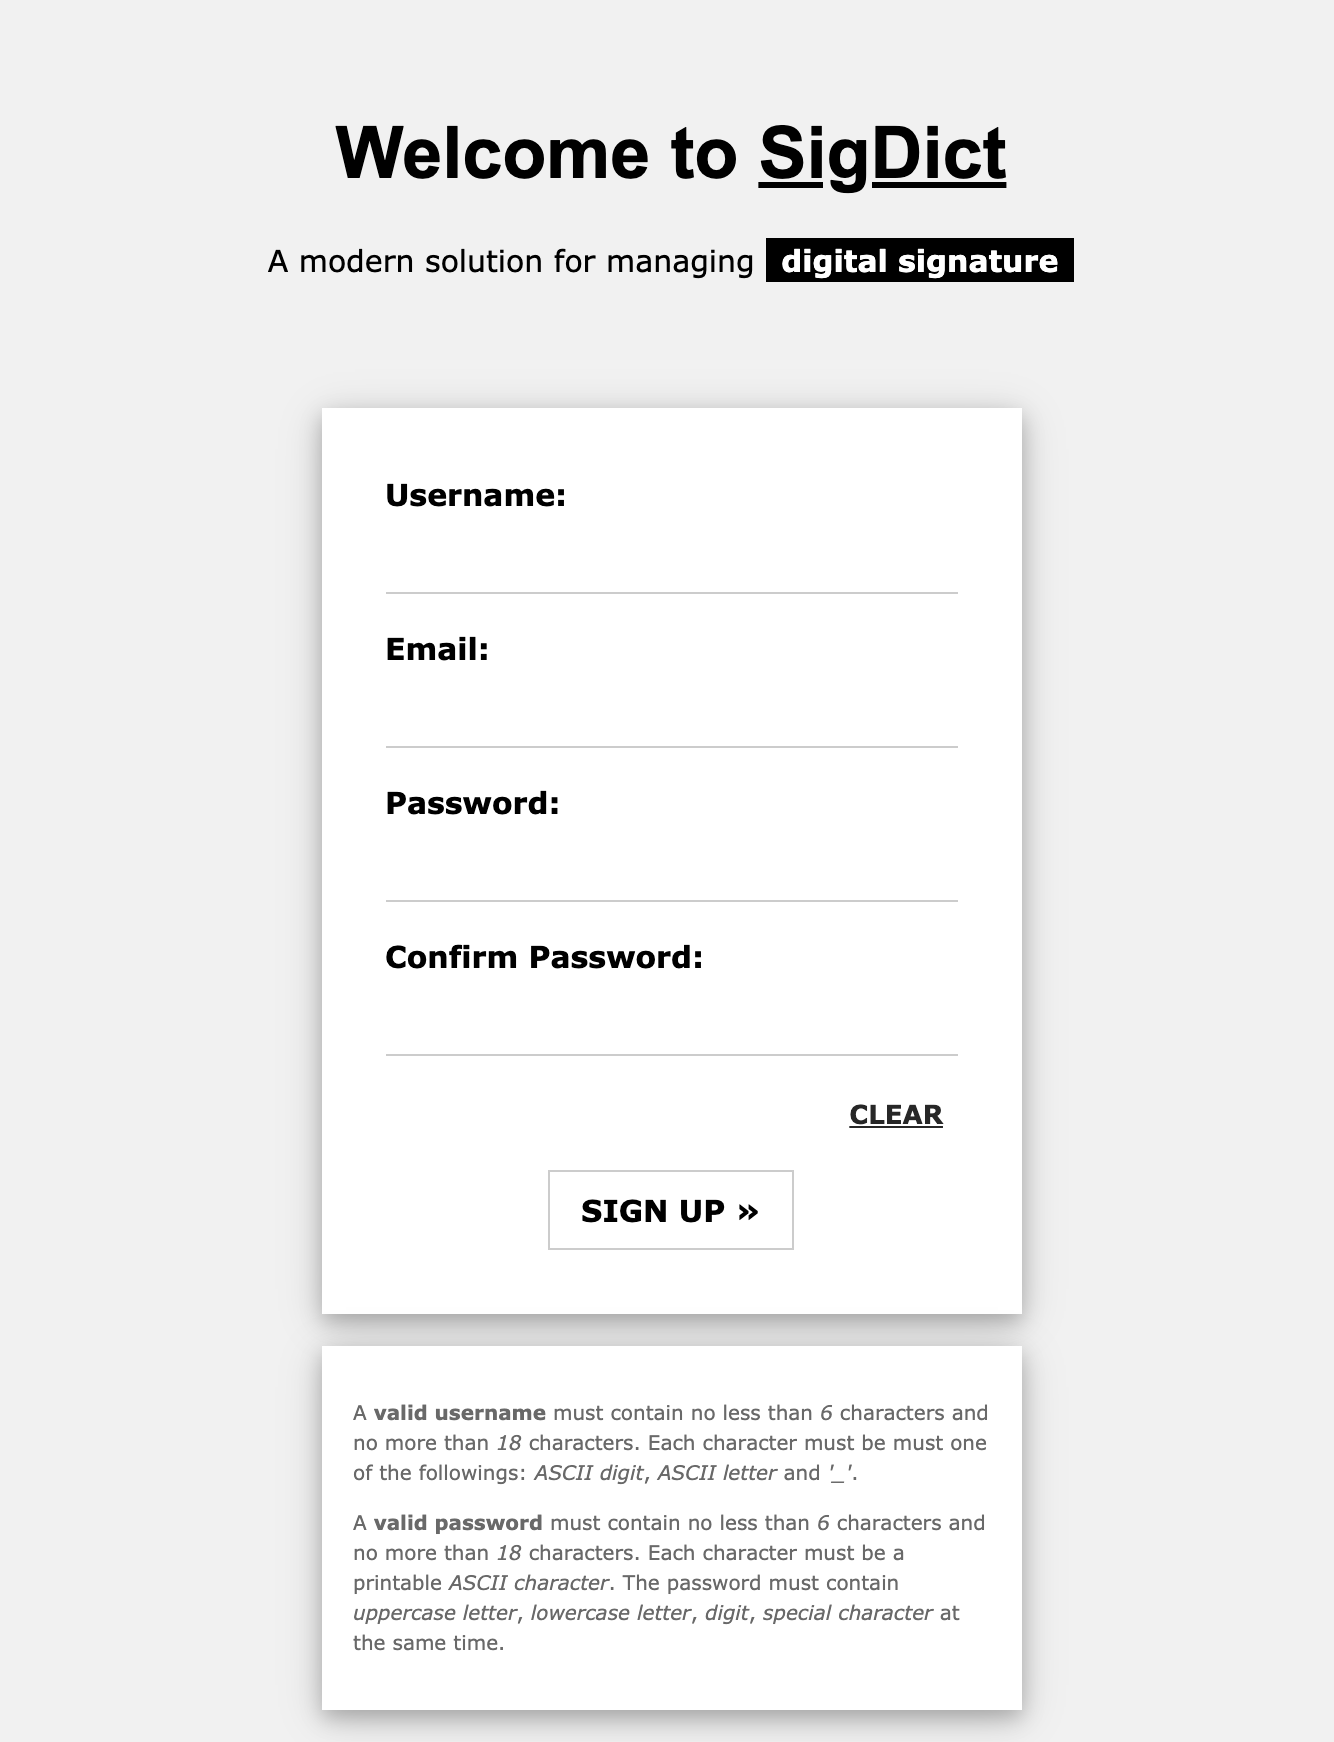
\includegraphics[width=1\textwidth]
		{figures/register.png}\\
		\caption{注册界面}
		\label{fig:register}
	\end{minipage}
\end{figure}

\section{主界面}

用户在登录后就可以进入自己的主界面,如图\ref{fig:main}所示。

在主界面的中间的模块中显示了当前用户的一些个人信息,例如用户名、电子邮箱地址等等。并且用户可以在这个模块中点击“SHOW”查看自己的DSA,RSA公钥信息。同时用户也可以在这个模块中完成更换密钥、更改电子邮箱地址、更改密码、登出等操作。其中更换密钥操作会让用户获得全新的、随机生成的密钥,并更新所有受到影响的文件的数字签名。

在本页面下方的模块中显示了用户所有上传的文件信息,包括上传时间、文件名称等数据段。同时可以通过点击“DETAIL”查看包含数字签名在内的文件的详细信息,如图\ref{fig:detail}所示。用户可以通过上方的搜索框,通过关键词搜索快速找到所需的文件。同时用户也可以选择上传、下载、删除某个特定的文件。

\begin{figure}[!htb]
	\centering
	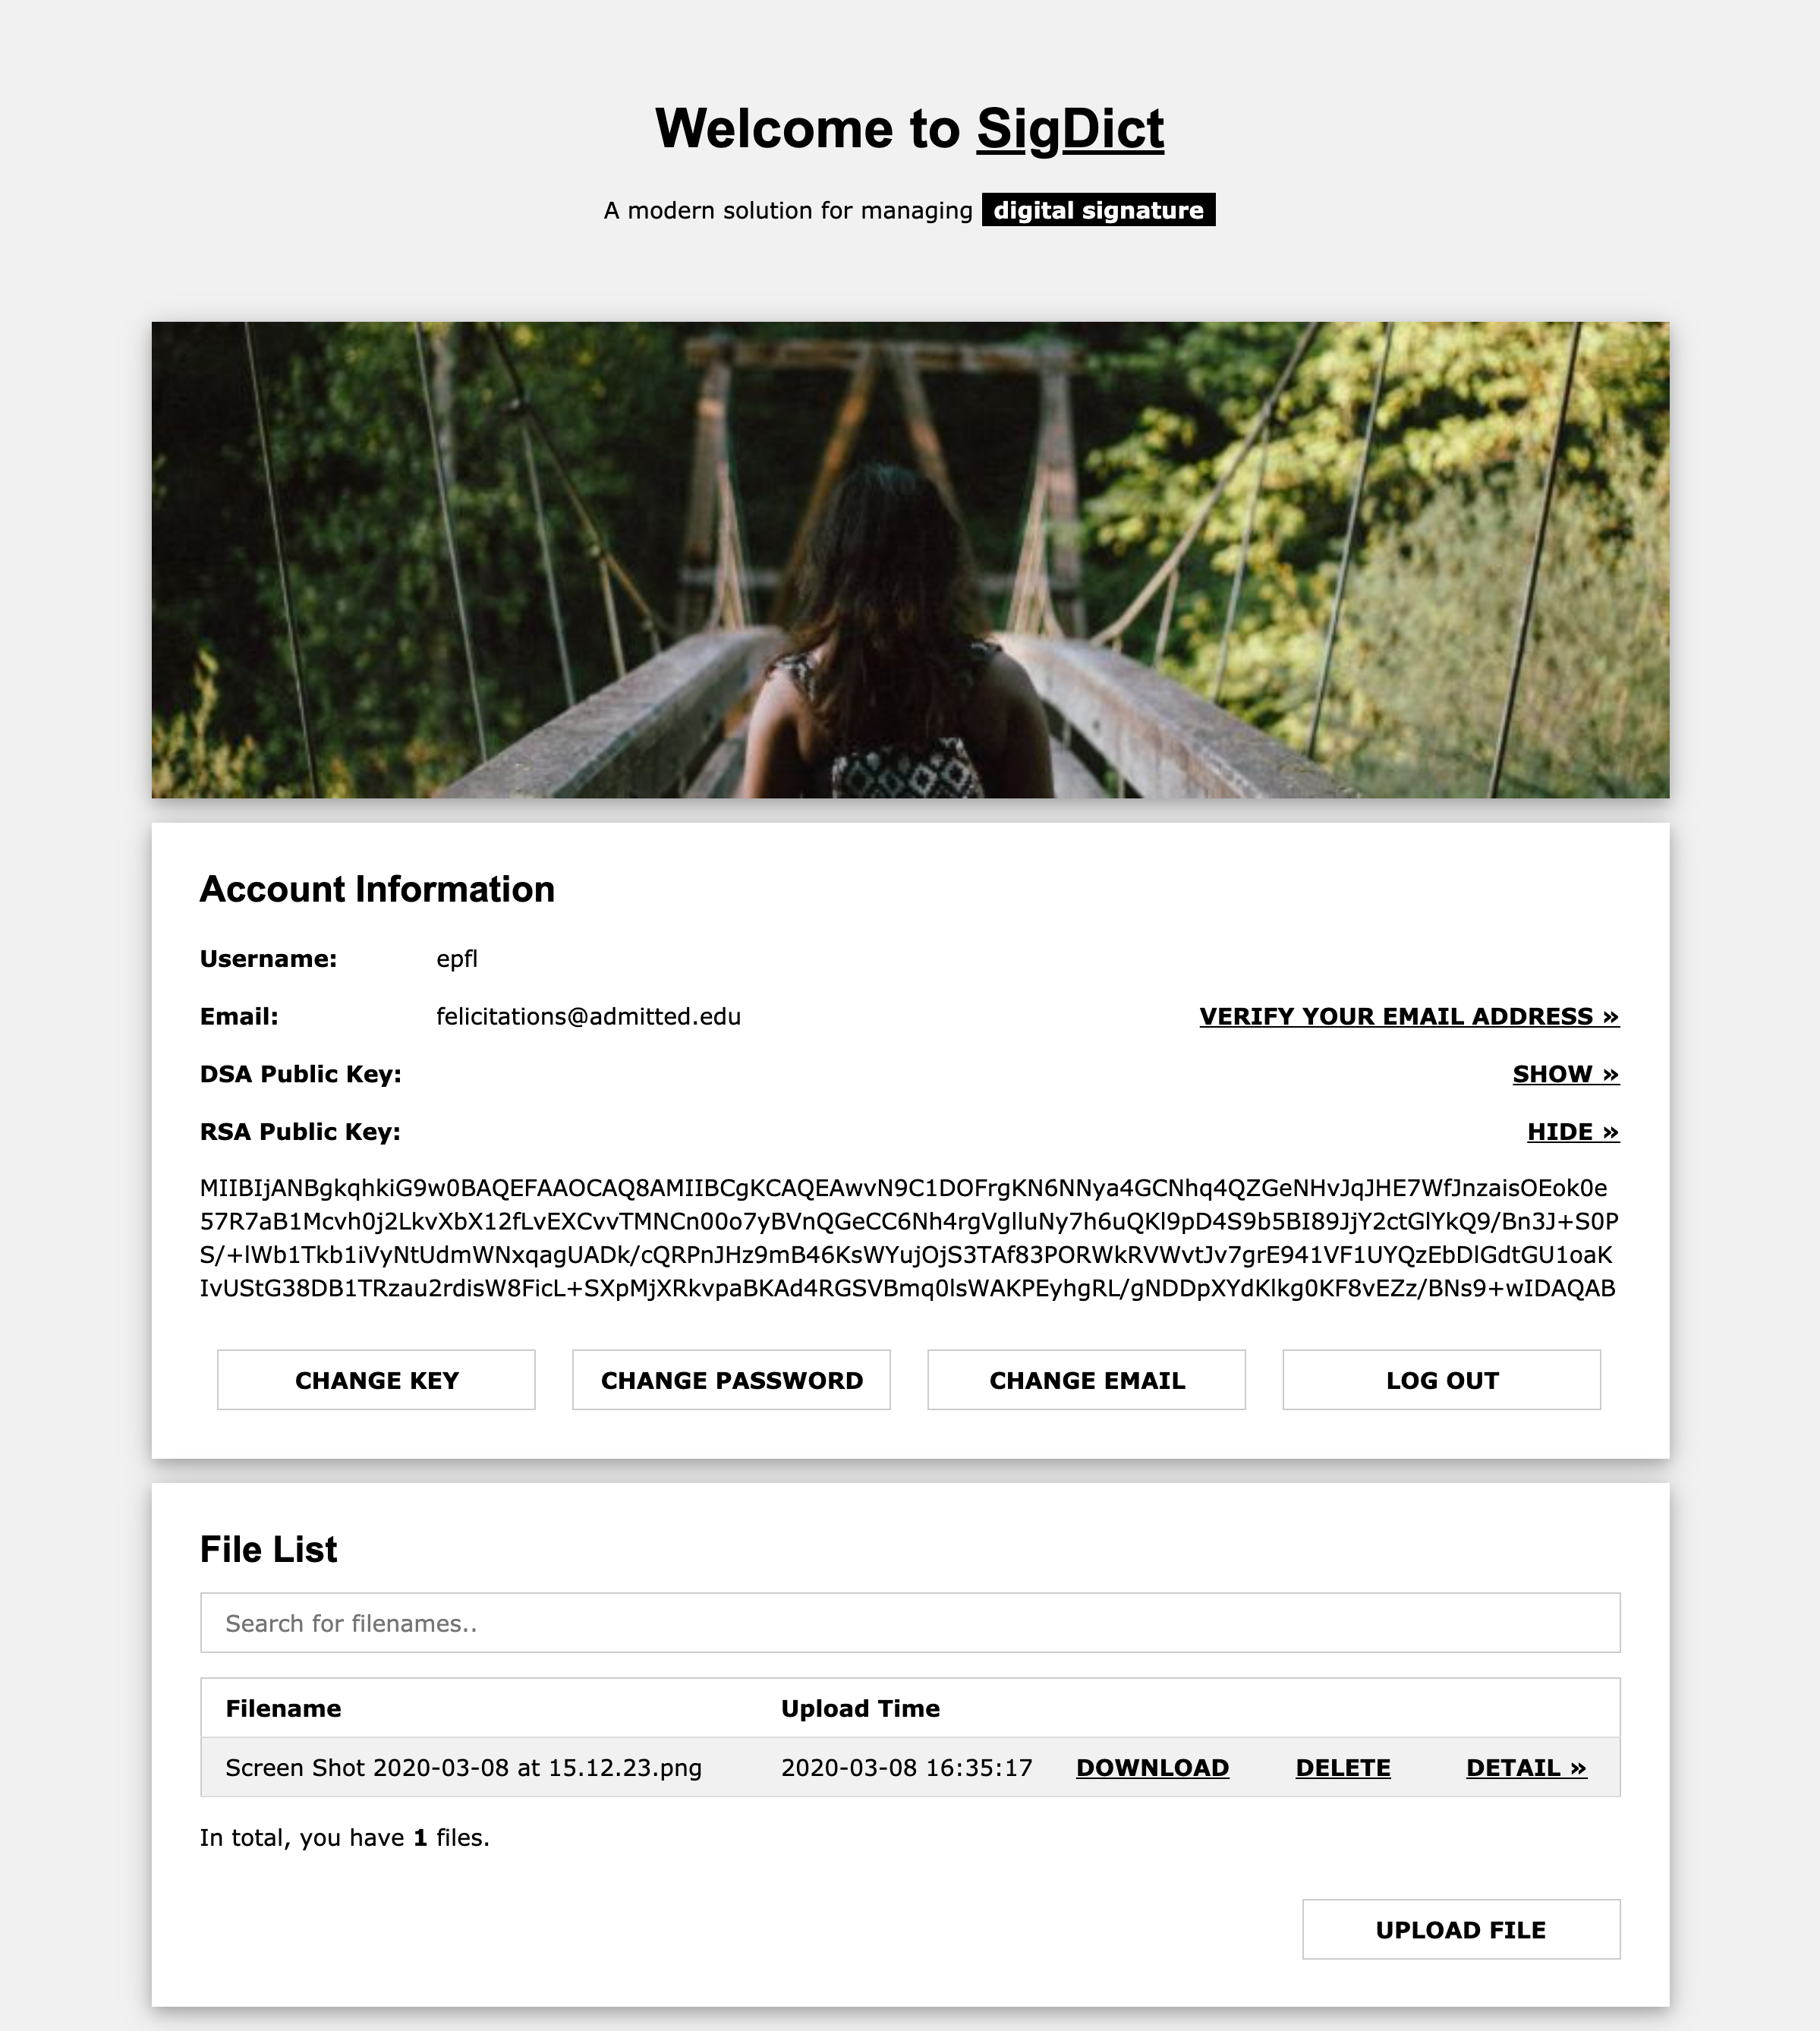
\includegraphics[width=0.8\textwidth]
	{figures/main.png}\\
	\caption{主界面}
	\label{fig:main}
\end{figure}

\section{上传界面}

如图\ref{fig:upload}所示,用户可以在该界面选择上传文件到网站中,并获得相应的数字签名信息。在上传文件的时候,用户可以选择用来进行签名的算法,我们现在提供DSA,RSA两种签名算法供用户使用,同时用户还可以选择勾选“ENCRYPT FILE”多选框,让文件以加密的形式存储在服务器中,提供更加安全的环境。同时为了确保上传文件的安全性,我们对可以上传文件的类型、大小进行了限制,见小节\ref{sec:fileV}。

\begin{figure}[!htb]
	\begin{minipage}[t]{0.5\textwidth}
		\centering
		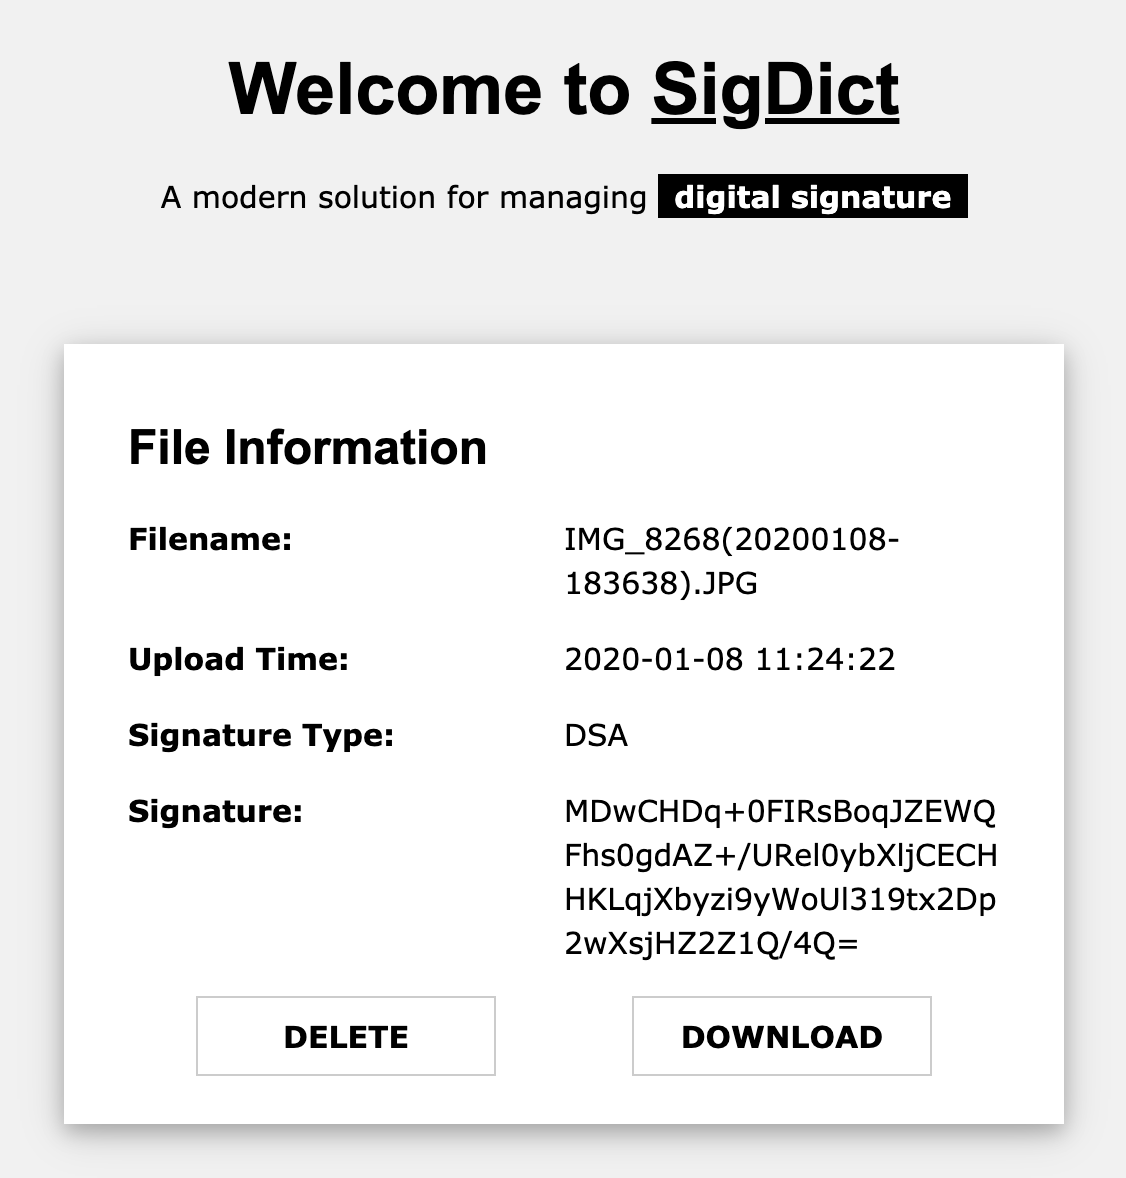
\includegraphics[width=1\textwidth]
		{figures/detail.png}\\
		\caption{详情界面}
		\label{fig:detail}
	\end{minipage}
	\qquad
	\begin{minipage}[t]{0.5\textwidth}
		\centering
		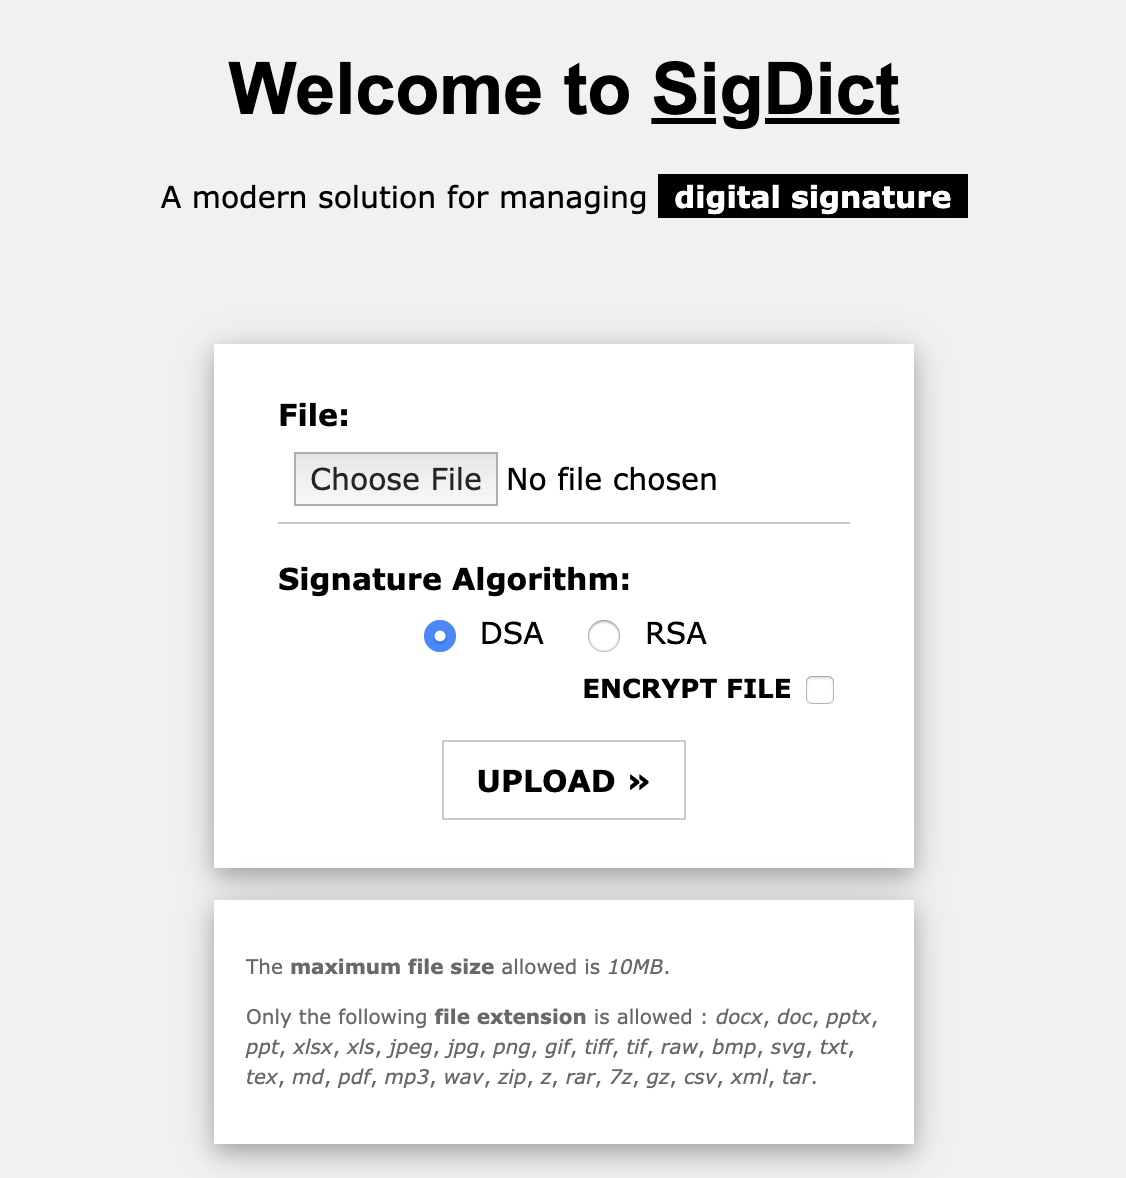
\includegraphics[width=1\textwidth]
		{figures/upload.png}\\
		\caption{上传界面}
		\label{fig:upload}
	\end{minipage}
\end{figure}


\section{忘记密码和重置密码界面}

如果用户忘记了自己的密码,在用户的邮箱已经通过了验证(见小节\ref{sec:emailV})的情况下,用户可以选择通过电子邮箱的方式重置密码。点击登录界面中的“FORGET PASSWORD”链接就可以跳转到图\ref{fig:forgetpassword}所示界面。在正确的填写相应信息后,一封包含重置密码链接的邮件会被发送到用户指定的电子邮箱中,同时页面会跳转到图\ref{fig:message}所示的信息页面中。用户点击电子邮件中包含的链接即可进入图\ref{fig:resetpassword}所示的重置密码页面,完成对密码的重置工作。

\begin{figure}[!htb]
	\begin{minipage}[t]{0.5\textwidth}
		\centering
		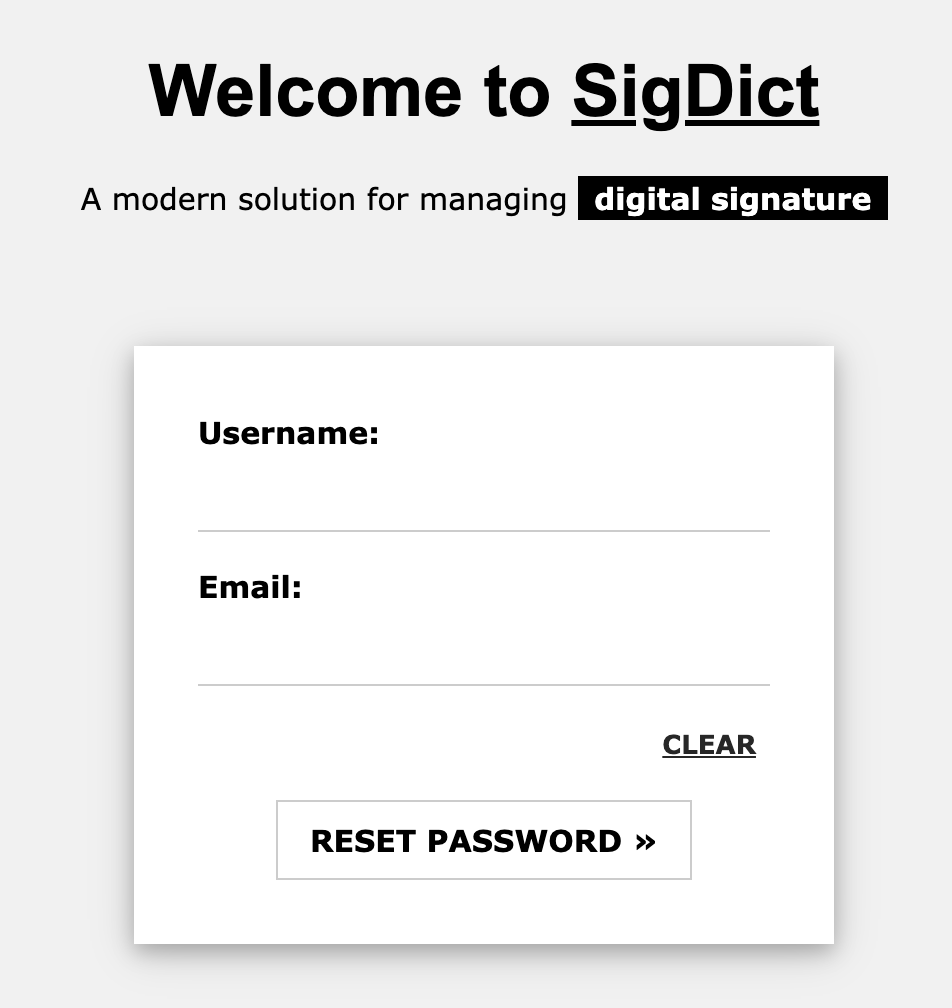
\includegraphics[width=1\textwidth]
		{figures/forgetpassword.png}\\
		\caption{忘记密码界面}
		\label{fig:forgetpassword}
	\end{minipage}
	\qquad
	\begin{minipage}[t]{0.5\textwidth}
		\centering
		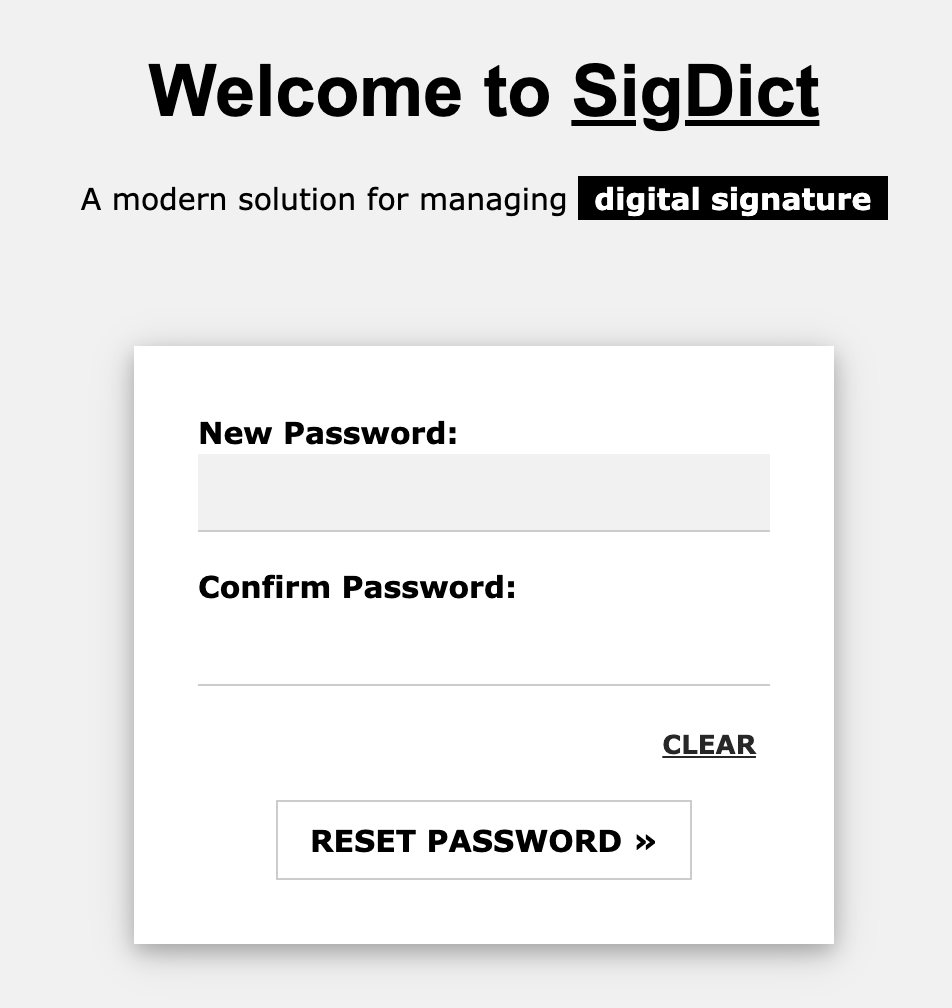
\includegraphics[width=1\textwidth]
		{figures/resetpassword.png}\\
		\caption{重置密码界面}
		\label{fig:resetpassword}
	\end{minipage}
\end{figure}

\section{消息和错误信息界面}

如图\ref{fig:message}所示,在发送重置密码链接、设置新密码的过程中服务器会通过重定向到消息界面的形式向用户传达一定的信息。

如图\ref{fig:error}所示,如果由于用户的错误操作,或者是服务器端的某些错误导致无法正常相应用户请求,用户会被重定向到错误信息界面中,并显示相应的提示信息。现阶段我们支持了以下几种类型的错误提示:

\begin{itemize}
	\item \textbf{400 BAD REQUEST}
	
	如果用户请求中的参数不齐全,或者参数格式、内容有误有可能会出发这个错误,造成服务器端无法正常响应。
	
	\item \textbf{404 NOT FOUND}
	
	如果服务器无法找到用户请求的资源,会触发该错误。
	
	\item \textbf{405 METHOD NOT ALLOWED}
	
	对于部分API接口,我们只允许用户用某些特定的方式访问,例如只允许post方式访问。如果用户的访问方式不正确会触发该错误。
	
	\item \textbf{500 INTERNAL SERVER ERROR}
	
	如果服务器内部出现了未catch的异常、崩溃、内存泄露等问题有可能会触发该错误。
	
	\item \textbf{UNKNOWN ERROR}
	
	对于一切其他原因导致的异常情况都会触发该错误。
	
\end{itemize}

\begin{figure}[!htb]
	\begin{minipage}[t]{0.5\textwidth}
		\centering
		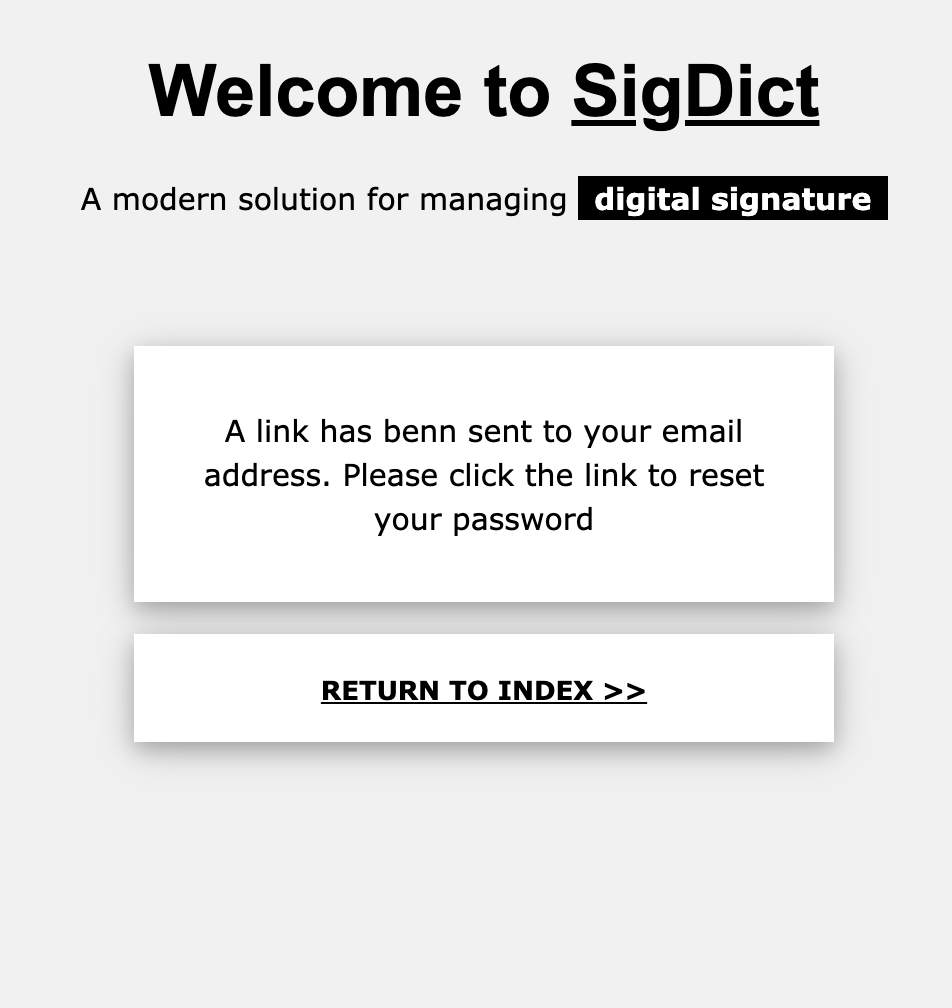
\includegraphics[width=1\textwidth]
		{figures/message.png}\\
		\caption{消息界面}
		\label{fig:message}
	\end{minipage}
	\qquad
	\begin{minipage}[t]{0.5\textwidth}
		\centering
		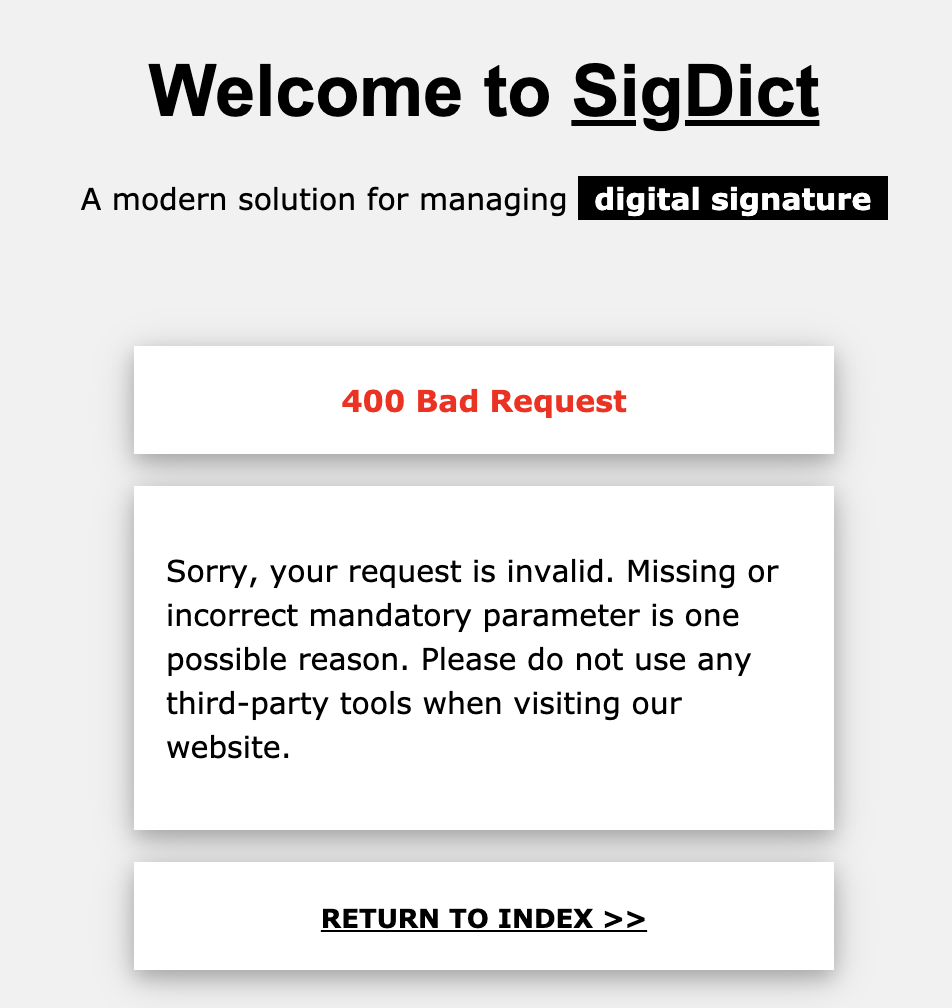
\includegraphics[width=1\textwidth]
		{figures/error.png}\\
		\caption{错误界面}
		\label{fig:error}
	\end{minipage}
\end{figure}


